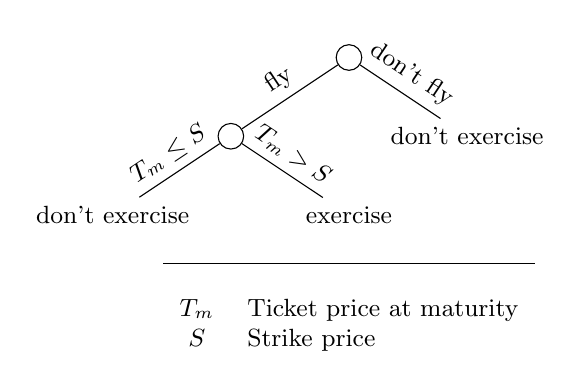
\begin{tikzpicture}[grow=down, sloped,
                    level 1/.style={sibling distance=3cm, level distance=1cm}, level 2/.style={sibling distance=3cm, level distance=1cm},
                    bag/.style={circle, draw, minimum width=1em}]
\small
\node[bag] {}
    child {
        node[bag] {}
        child {
                node[align=center] {don't exercise}
                edge from parent
                node[above] {$T_m \le S$}
            }
            child {
                node[align=center] {exercise}
                edge from parent
                node[above] {$T_m > S$}
            }
        edge from parent
        node[above] {fly}
    }
    child {
        node {don't exercise}
        edge from parent
        node[above] {don't fly}
    };

\node at (0,-3.2)
{
\begin{tabular}{cl}
\hline \\
$T_m$ & Ticket price at maturity \\
$S$ & Strike price
\end{tabular}
};
\end{tikzpicture}
